\subsection{Real Data}
Below, we present the results of running the algorithm on several real life datasets. Merchants 1 and 2 have on the order of 25k products with 250k relations between them while Merchants 3, 4 and 5 have on the order of 250k products with 2.5m relations between them. The size of the true optimal solution was unknown to us, and we estimated this quantity by taking the minimum of $|L|c/a$ and the number of vertices in $R$ of degree at least $a$. Note that this is an upper bound on OPT, and that it's almost certain that the true OPT is lower than this value. We could not run the partition algorithm for Merchants 3, 4 and 5 due to memory constraints.

\begin{figure}[t]
\centering
\begin{minipage}[h]{0.48\textwidth}
\centering
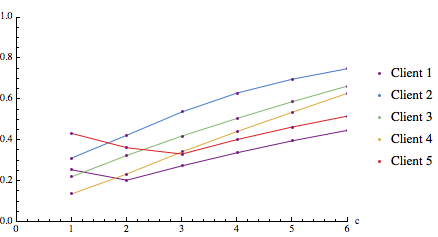
\includegraphics[width=0.8\textwidth]{images/real_sampling_a=1.png}
\caption{Sampling algorithm for different values of $c$ when $a=1$}\label{fig:real_sampling_a=1}
\end{minipage}
\hspace{0cm}
\begin{minipage}[h]{0.48\textwidth}
\centering
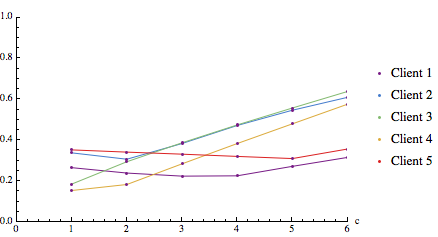
\includegraphics[width=0.8\textwidth]{images/real_sampling_a=2.png}
\caption{Sampling algorithm for different values of $c$ when $a=2$}\label{fig:real_sampling_a=2}
\end{minipage}
\hspace{0cm}
\centering
\begin{minipage}[h]{0.48\textwidth}
\centering
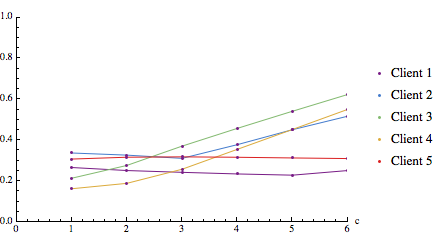
\includegraphics[width=0.8\textwidth]{images/real_sampling_a=3.png}
\caption{Sampling algorithm for different values of $c$ when $a=3$}\label{fig:real_sampling_a=3}
\end{minipage}
\vspace{-0.2in}
\end{figure}

\begin{figure}[t]
\centering
\begin{minipage}[h]{0.48\textwidth}
\centering
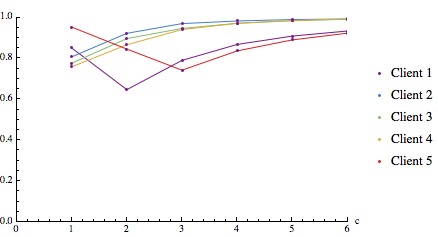
\includegraphics[width=0.8\textwidth]{images/real_greedy_a=1.png}
\caption{Greedy algorithm for different values of $c$ when $a=1$}\label{fig:real_greedy_a=1}
\end{minipage}
\hspace{0cm}
\begin{minipage}[h]{0.48\textwidth}
\centering
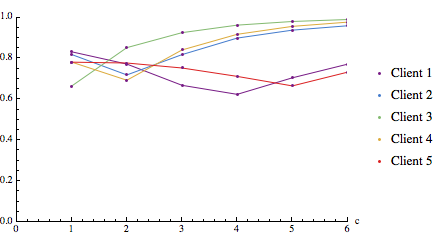
\includegraphics[width=0.8\textwidth]{images/real_greedy_a=2.png}
\caption{Greedy algorithm for different values of $c$ when $a=2$}\label{fig:real_sampling_a=2}
\end{minipage}
\hspace{0cm}
\begin{minipage}[h]{0.48\textwidth}
\centering
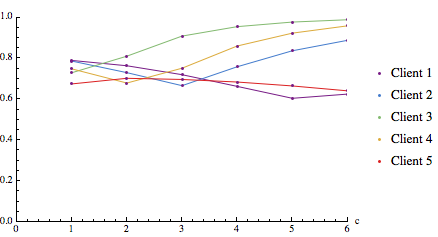
\includegraphics[width=0.8\textwidth]{images/real_greedy_a=3.png}
\caption{Greedy algorithm for different values of $c$ when $a=3$}\label{fig:real_greedy_a=3}
\end{minipage}
\vspace{-0.2in}
\end{figure}

From these results, we can see that that greedy performs exceptionally well when $c$ gets even moderately large.
For realistic value of $c=6$, greedy performed better than 85\% optimally for Merchants 2, 3 and 4. For Merchants
1 and 5, the results were less optimal but still quite promising since the algorithm still performed 60\% optimally.
The sampling algorithm also does in real life data, but only when $c$ get rather large. It is therefore impractical
to use on all but the largest of data sets that can't even pay the $O(|L|+|R|)$ memory cost of the greedy algorithm.